\chapter{Configuración Wi-Fi}
Wi-Fi permanece apagado durante el funcionamiento normal. Mantenga el teléfono a unos 10–20 cm del indicador durante la configuración. La contraseña predeterminada es 1234567890 y la dirección del panel es http://192.168.4.1.

Con USB desconectado, encienda el contacto o la alimentación e inmediatamente pulse el botón trasero. Aparecerá un código QR. Desactive los datos móviles, escanee el código y conecte el teléfono a la red Wi-Fi del indicador. Abra el panel en el navegador, seleccione la aplicación y el sensor correspondiente, guarde y apague y encienda el contacto.

Si no puede acceder, acerque el teléfono y compruebe que sigue conectado a la red del indicador aunque no tenga Internet. Repita el arranque con QR si es necesario. El botón trasero también sirve para interactuar con las aplicaciones y seleccionar el modo de arranque durante la programación inicial.

USB está previsto para la programación inicial; para actualizaciones posteriores se recomienda la interfaz web. Desconecte todo el cableado del vehículo antes de usar USB. Siga las instrucciones de la versión de firmware; la fuente no detalla un procedimiento de recuperación ni un menú de carga.

\begin{figure}[H]
\centering
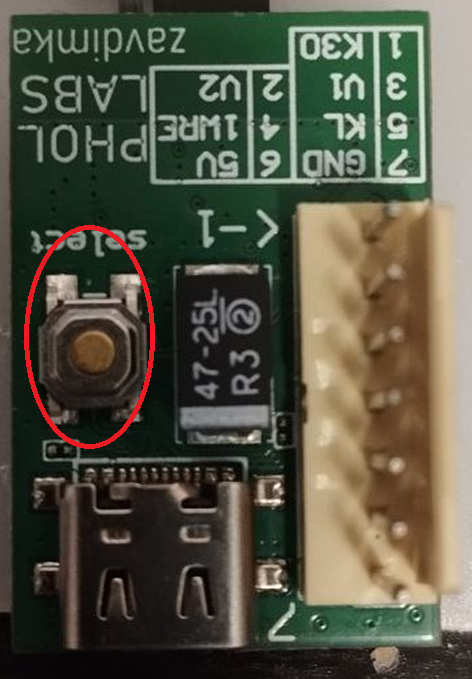
\includegraphics[width=.85\textwidth,height=.60\textheight,keepaspectratio]{figures/ivevo/image11.png}
\caption{Configuración Wi-Fi}
\end{figure}
